%Observations of low redshift galaxies have established a relationship between galaxy stellar mass, metallicity, and SFR, controversially ref called the "fundamental relation" (Ellison+2008, Mannucci+2010, LaraLopez+2010). At redshifts between 1 and 3, the nature of the FMR is uncertain. Some studies find a constant FMR at all metallicities (Wuyts et al. 2012,Henry et al. 2013; Hunt et al. 2016) while others find a FMR that evolves with redshift (Zahid et al. 2014; Grasshorn Gebhardt et al. 2016; Kashino et al. 2017).
%Our understanding of gas properties in the earliest galaxies remains primitive. This is exacerbated by our lack of tools; at redshifts above $z{\sim}5$, the well-established optical diagnostics are observationally inaccessible with ground-based optical and IR facilities. To probe the physical conditions of the gas in these early galaxies, we must instead rely on emission line diagnostics that originate in the ultra-violet (UV) part of the spectrum.


\section{UV-derived metallicities}\label{sec:UVZ}

In this section, we derive metallicities for the \mage galaxies using the most promising set of diagnostics from \S\ref{sec:ZZ:UV}. The \mage galaxies with both UV and optical metallicities can be used to connect studies where only optical or only UV metallicities are available. We first derive metallicities using all 12 diagnostics used in this work. We then propose a new weighting scheme based on the post promising subset of diagnostics identified in \S\ref{sec:ZZ:UVOpt}, and then calculate UV metallicities for the \mage sample.

Fig.~\ref{fig:UVmage} shows the gas phase oxygen abundance derived using all 12 UV diagnostics for each of the \mage galaxies. Each point is color-coded by the diagnostic used to derive the abundance, using the same scheme as Fig.~\ref{fig:UVZ}, as indicated in the color bar. The diagnostics predict oxygen abundances between $7.75< 12+$\logOH$<8.75$. The spread in predicted metallicities for a given object varies between 0.25 dex and 0.75 dex.

As expected, in Fig.~\ref{fig:UVmage}, the Si2Si2-Si2Si3 diagnostic (pale blue diamonds) predicts the largest oxygen abundances in every object, offset from other predictions by at least $\sim0.25$ dex, and in an extreme case, by as much as 1\,dex. The metallicities predicted with this diagnostic exceed solar metallicity in most cases, which corresponds to gas enrichment that may be difficult to attain at the metallicities in this sample.

The best of the diagnostics identified in \S\ref{sec:ZZ:UV} included Si2Si2-O3Si3 (bright green diamonds), Si2O3-Si3O2 (brown), Si2Si2-N3Si3 (pale orange), and Si2Si2-O2O3 (pale red). When simultaneously measured in a single object, the spread in predicted metallicity is small, as expected.

From our analysis in \S\ref{sec:ZZ:UVOpt}, Si2Si2-O3Si3, Si2O3-Si3O2, Si2Si2-N3Si3, and Si2Si2-O2O3 produce the most accurate and precise metallicity estimates. To calculate a final UV metallicity for the galaxies in the \mage sample, we thus propose a weighted average of the metallicities derived with these four diagnostics, following the form \XXX; these metallicities are given in Table.\XXX.

Fig.~\ref{fig:UVmage} shows the "final" UV metallicity calculated for each of the \mage galaxies, now plotted as a function of redshift. For comparison, we also compare the metallicities and redshifts from blah (\XXX actually make this plot; not sure if this is the best way to summarize results).

%-------------------------------------------------------
% Figure 8:
%-------------------------------------------------------
\begin{figure*}
  \begin{center}
    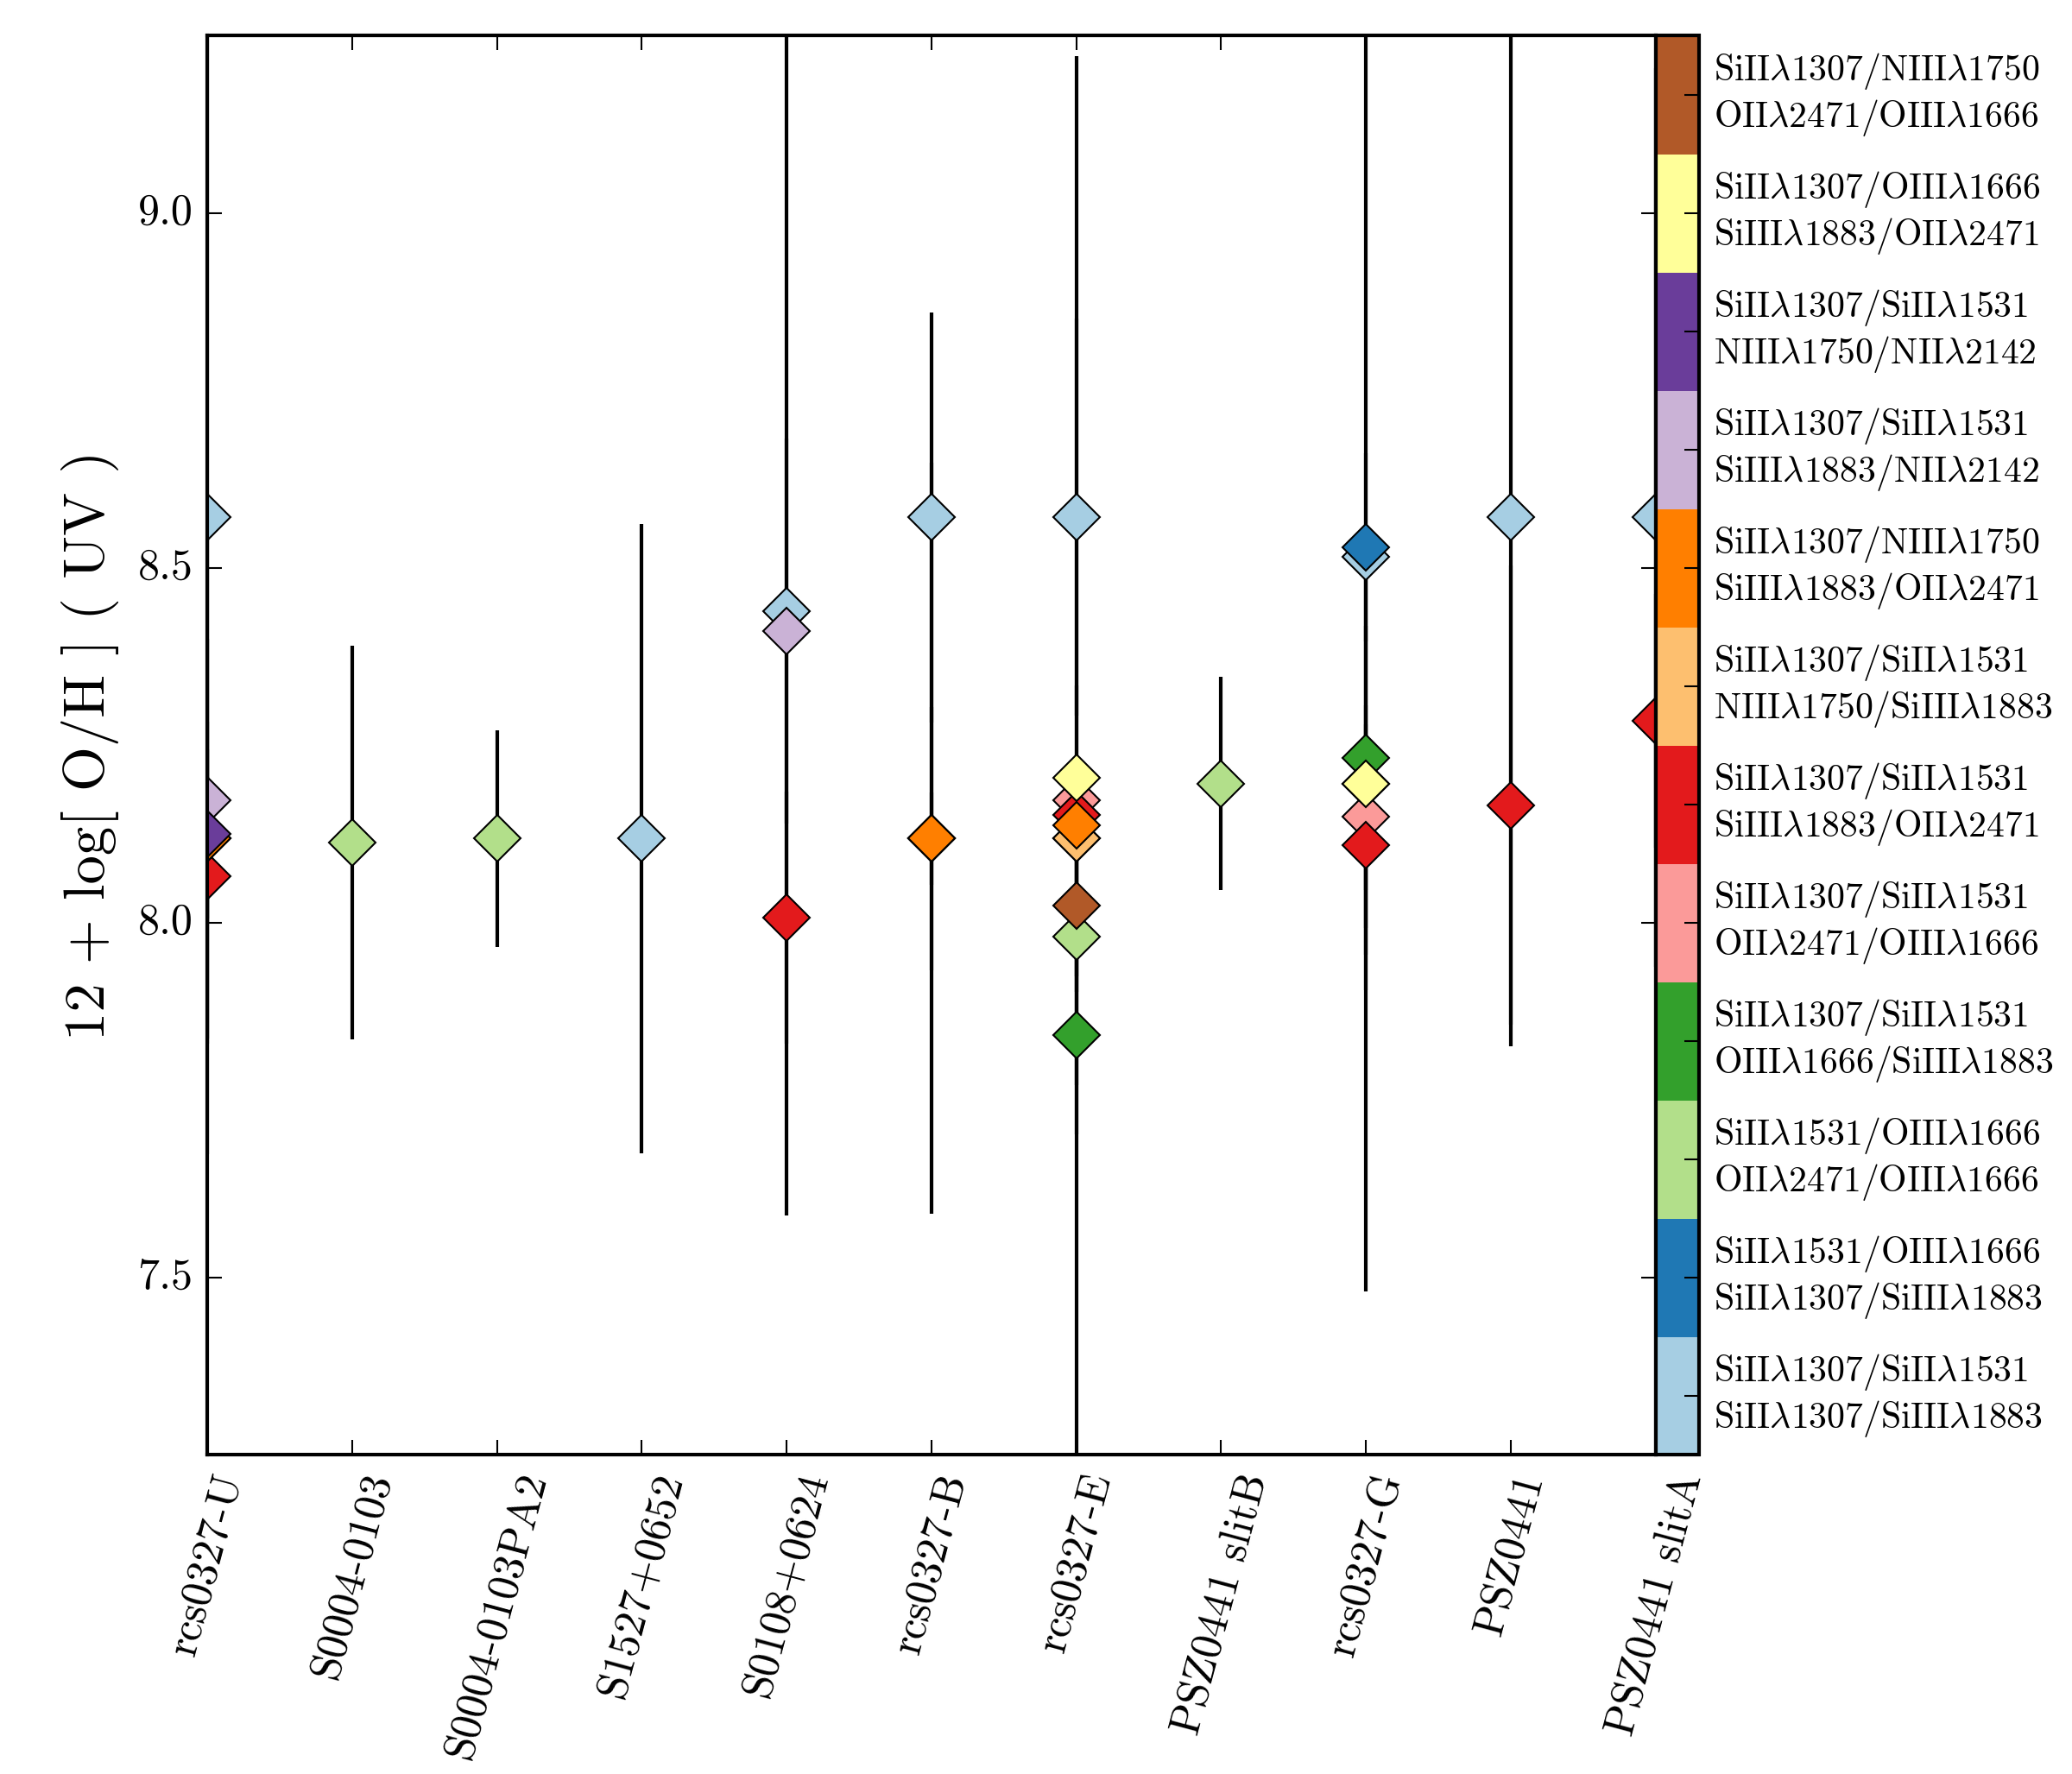
\includegraphics[width=\linewidth]{figs/f8.png}
    \caption{UV-derived metallicities ($y$-axis) for the \mage galaxies, each object is offset on the $x$-axis arbitrarily. Each marker is is color-coded by the diagnostic diagram used to derive the metallicity, as shown in the colorbar. }
    \label{fig:UVmage}
  \end{center}
\end{figure*}
%-------------------------------------------------------